
\section{はじめに}

いろはかるた，競技かるたのように，音声を手がかりに進む遊びでは，字幕を使って音声の内容を伝えることがある．しかし，字幕を音声の各文字の開始時刻に合わせて表示するだけでは，音声と文字で分かっていく過程や分かるタイミングまで揃うとは限らない．また，ドラマの字幕や音楽の歌詞でも，音声より先に文字が表示され，文字から先に内容を識別できることがある．そのため，音声を聞きながら少しずつ内容が分かっていくという，言葉を聞く体験を字幕では保ちにくい．

そこで本研究では，文字の見え方を時間とともに変えることで，文字の識別過程をデザインできる動的フォント timeFont を提案し，その生成システムを実装した．音声や文字を途中まで提示したときに，何の文字かをどの程度識別できるかは，時間とともに変わる．本論文では，この時間変化を識別過程と呼ぶ．本システムは，かなの文字列から生成する方法と，既存の音声と識別データから生成する方法の 2 通りに対応する（図 1）．後者では，競技かるたで実測した決まり字の識別時刻 \cite{maruyama} など，本研究とは別に測定されたデータも利用できる．

本研究の貢献は，timeFont とその生成システムの実装，4 種類の表示方式についての対応データの構築，および生成した表示の一対比較による評価の 3 点である．2 章で関連研究を，3 章で timeFont とその考え方を述べる．4 章では timeFont を作るために必要な測定を行い，5 章では測定した結果から timeFont を作る手順を示す．6 章では作成した timeFont を評価する．7 章で使うためのツールと実装例を8章で今後の展望を述べる．


\begin{figure}[tb]
\begin{center}
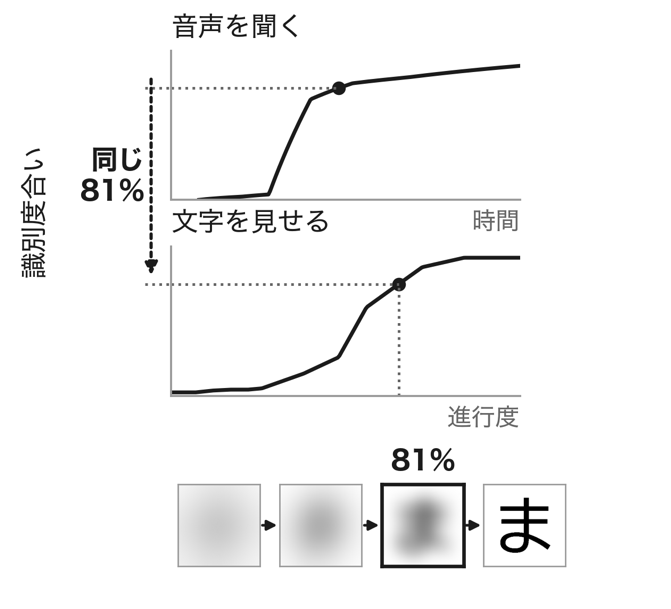
\includegraphics[width=0.70\hsize]{fig/fig1_concept.png}
\end{center}
\caption{timeFont 生成システムの入力と出力．}
\label{fig:concept}
\end{figure}

\section{関連研究}

刺激を途中まで提示し，その時点で何であるかを回答させる方法は，音声知覚で用いられてきた．日本語でも，単音節の分割や，連続音声から切り出した音節の知覚実験が行われている \cite{takeuchi,kuwahara,katagiri}．Grosjean \cite{grosjean} は，単語を先頭から徐々に長く提示するゲーティング法を用いて単語認識の過程を調べた．Furui \cite{furui} は日本語音節を前後から打ち切り，正答率が急に変わる時点とスペクトル遷移との関係を調べている．また Smits \cite{smits} は，調音様式，調音位置，有声性によって識別情報の時間分布が異なることを示した．本研究ではこの違いを考慮し，音の種類によって提示時点を設定した．

視覚については，Petersen and Andersen \cite{petersen} が，1 文字の提示時間と識別率の関係を測定している．Sánchez-García ら \cite{sanchez} は，音声と視覚発話を時間方向に打ち切り，音素識別の時間変化を測定した．これらが提示量と識別の関係を測定しているのに対し，本研究では，測定した関係を生成に用い，目標とする識別の時間変化に対応する文字の表示状態を求める．

動的な文字表示については，Braggら\cite{bragg} がアニメーションを用いた書体 livefonts を提案し，従来の書体のおよそ半分の面積でも判読できることを示した．Lee ら \cite{lee} は，複数の時間変化を組み合わせて文字アニメーションを生成する kinetic typography engine を提案している．植月ら \cite{uetsuki17} は，コントラストが時間とともに変化する文字について提示速度と読みの特性を調べ，さらに発話の速度や間を文字の時間変化として表す textual prosody を検討している \cite{uetsuki20}．また de Lacerda Pataca and Costa \cite{pataca} は，音声の大きさ，高さ，長さを，文字の太さ，位置，字間へ対応づけている．これらに対し本研究では，音響的な特徴そのものではなく，音声と文字を途中まで提示したときの識別の変化を対応づけ，目標とする識別の時間変化から文字の表示状態を求める．著者らが別に測定した競技かるたの識別時刻 \cite{maruyama} も，外部から与える目標として利用できる．我々が調査した範囲では，目標とする識別の時間変化と，文字の提示状態から得た識別率の対応を用いて文字アニメーションを生成する手法は確認できなかった．


\section{timeFont とは}

timeFont は，文字ごとに，どの時刻にどこまで表示を進めるかを決め，それに従って表示を連続的に変えていく動的なフォントである．表示の途中の状態は 0 から 100\% の進行度で表す．同じ手法は任意の文字列にも適用可能である．

音声と文字アニメーションを対応づけるには，両者に共通して測れる量が必要である．本研究では，刺激を途中まで提示して何の文字かを答えてもらう同じ形式の課題を，音声と文字の両方に対して行う．その回答から，何の文字であるかを当てられた割合（正答率）と，回答の散らばりから求めた情報量の 2 つが得られる．どちらも識別がどこまで進んだかを表す量であり，音声でも文字アニメーションでも同じように測れる．たとえば音声を 20 ms まで提示したときの正答率が 76\% であれば，同じ時刻の文字アニメーションを，正答率が 76\% となる進行度まで進める．

生成には，音声側と文字側の 2 本の曲線を用いる．音声を先頭から t ms まで提示して打ち切ったときの値と，文字アニメーションを進行度 s（\%）まで進めて打ち切ったときの値を測定し，各時刻で同じ値になる進行度を求める．以下では，この課題を測定と呼ぶ．4 章と 5 章では正答率を用い，6 章で情報量を用いた場合と比べる．

本研究では次の 3 つを明らかにする．(1) 音声と文字アニメーションの識別過程を，測定にもとづいて対応づけられるか．(2) 対応のつき方は表示方式によってどう違うか．(3) 対応づけに用いる量（正答率か情報量か）によって，生成された表示の評価は変わるか．


\section{timeFont を作るための測定}

3 章の手順は，音声を途中で止めたときの正答率と，文字アニメーションを途中で止めたときの正答率が，どちらも分かっていることを前提とする．この正答率は，文字によっても表示方式によっても違うため，測ってみなければ分からない．そこで，各文字・各表示方式について，進行度と正答率の対応を測った．測定は聴覚と視覚の 2 条件で行った．いずれの条件でも，途中で打ち切って提示した刺激に対し，実験協力者はかな表から 1 文字を選んで回答する．この回答の正答率から$A_i(t)$と，表示方式ごとの $V_i(s)$を求めた．本研究では，聴覚の測定，視覚の測定，および生成した表示の一対比較の 3 つを，それぞれ異なる実験協力者に対して行った．応募の時点で過去の参加履歴を照合し，いずれかにすでに参加していた場合は参加対象外とした．実験協力者は Yahoo! クラウドソーシングで募集し，日本語母語話者，18 歳以上，各条件 1 人 1 回を条件とした．刺激を打ち切らずに全部提示する問題を試行に混ぜ，これを一定の割合で誤った実験協力者は分析から除外した．この基準により，聴覚 1 名，視覚 6 名を除外した．正答率の差は，参加者単位で再標本化するブートストラップにより求め，複数の比較を行うときの p 値は Holm 法で調整した．各試行では，提示条件と閲覧環境を記録した．


\subsection{表示方式}

本研究で実装した 4 つの表示方式では，各表示状態を 0 から 100\% の進行度で表し，式 (1) で求めた進行度に従って表示を変化させた．文字の見え方を時間とともに変化させる方法は複数考えられる．そこで本研究では，見え方の変え方が互いに異なる 4 つの表示方式を実装し，どの方式でも同じ手順で生成できるようにした．フェード方式は文字全体を薄い状態から濃くし，部分表示方式は画素を無作為な順に加え，ぼかし解除方式は強いぼかしを弱め，ワイプ方式は左から右へ描画領域を広げる．これらを図 2 に示す．部分表示の画素の順は文字ごとに固定した乱数順とし，ワイプの走査方向は全文字で左から右とした．方式ごとに測定した曲線の違いについては後述する．


\begin{figure}[tb]
\begin{center}
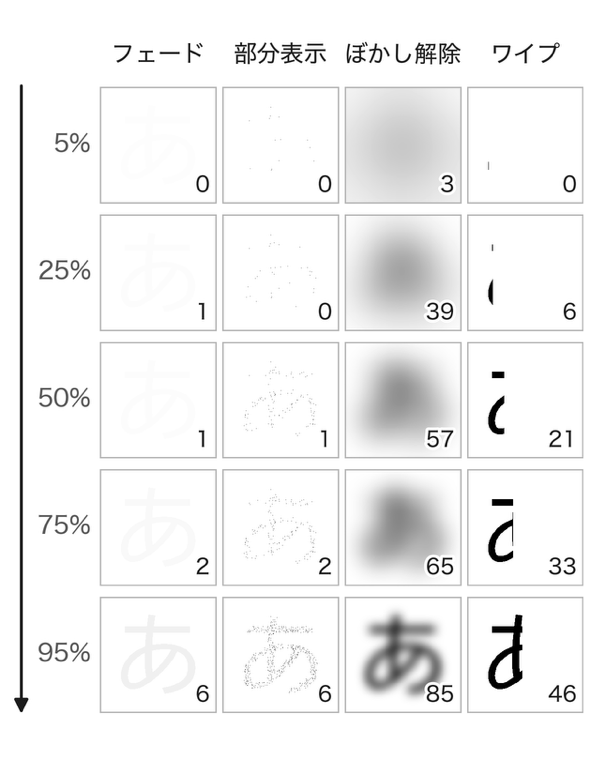
\includegraphics[width=0.62\hsize]{fig/fig2_families.png}
\end{center}
\caption{実装した 4 種類の表示方式．文字「あ」について，同じ正答率になる状態を並べた．数字はその状態の進行度（\%）である．}
\label{fig:families}
\end{figure}

\subsection{実験協力者と刺激}

対象は 8 文字とした．識別に必要な時間が異なると考えられる音を含めるため，音声学的な分類にもとづいて「あ」「か」「が」「ぱ」「し」「つ」「ま」「ら」を選んだ．これらは，母音（あ），軟口蓋無声破裂音（か），軟口蓋有声破裂音（が），両唇無声破裂音（ぱ），摩擦音（し），破擦音（つ），鼻音（ま），はじき音（ら）をそれぞれ含む．8 文字は，刺激の作成と測定に先立って固定した．

音声刺激は，音声合成（COEIROINK v2，話者「あみたろ」）で作成した．かな 1 文字だけを合成すると音声の長さが 1 秒前後まで伸びるため，各かなに後続モーラ「さ」を加えた 2 モーラの無意味語を作成し，全 68 かなについて合成したうえで，第 1 モーラだけを切り出した．切り出した第 1 モーラの長さは 77 から 164 ms（中央値 104 ms）であり，音量はそろえた．時刻 0 は音響信号の開始点とした．刺激は一度だけ提示し，実験協力者は五十音表と同じ並びのかな表から 1 文字を選んで回答する．回答してから次の試行を始めるため，試行のあいだには回答に要する時間が入る．回答の選択肢は聴覚条件で 68 文字，視覚条件で 72 文字と異なるが，偶然に正答する確率の差は 0.08 パーセントポイントにとどまるため，正答率をそのまま対応づけに用いた．


\subsection{提示時点と水準の配置}

提示時点は文字ごとに 7 点とし，打ち切らずに最後まで提示する条件を 1 点加えて 8 点とした．この時間の区切りは，識別情報の時間分布が音の種類によって異なるという知見 \cite{furui,smits} にもとづき，音の種類ごとに決定した．最短は 10 ms であり，最終時点は文字により 60 から 125 ms である．各実験協力者には 8 時点のうち 3 時点を割り当てる不完全ブロック計画とし，参加者間で 8 時点すべてのデータが得られるようにした．出題には，対象 8 文字と同じ回数だけ，それ以外の文字も提示した．視覚条件の進行度は，各表示方式について 8 水準を設定した．同じ進行度でも表示方式によって識別の難しさが大きく異なり，共通の水準を用いると多くの条件で正答率が下限または上限付近となり，中間域を十分に測定できないためである．


\subsection{進行の速さの 2 水準}

等速アニメーション全体の提示時間を 300 ms と，その約 1.67 倍にあたる 500 ms の 2 水準とし，同じ進行度を 300 ms 条件と 500 ms 条件の両方で測定した．これは，進行度と正答率の関係が提示時間によって変わるかを調べるためである．生成に用いる曲線は，提示時間の影響が認められた部分表示方式についてのみ 300 ms の試行に限って推定し，他の 3 方式は 2 条件を統合して推定した．端末の画面更新周期が異なっても指定した進行度のフレームが必ず 1 回は表示されるよう，そのフレームを少なくとも 1 フレーム描画したうえで刺激を消去した．


\subsection{得られた正答率曲線}

測定は聴覚 90 名，視覚 325 名で実施した．視覚は 2 回に分けて実施し，2 回目ではぼかし解除方式とワイプ方式の提示水準を変更した．1 回目と 2 回目の実験協力者も互いに異なる．生成に用いる曲線は，いずれの方式も 2 回で測った水準を合わせて求めた．

聴覚では，各提示時点をおよそ 30 試行で測定した（正答率 50\% 付近での二項比率の標準誤差はおよそ 9 パーセントポイント）．最後まで提示した条件の正答率は，「あ」と「か」で 94\% と高い一方，「し」で 43\%，「が」で 3\% にとどまった．

視覚では，4 つの表示方式すべてについて進行度と正答率の対応を得た．生成には，文字ごとの曲線 $V_i(s)$ を用いる．

フェード方式は不透明度が 256 階調で表現されるため，進行度 0.8\% が不透明度の整数値 2，1.4\% 前後が 3 に相当し，その間の水準は設定できない．実際の測定でも，進行度 0.8\%（正答率 14.6\%）から 1.4\%（同 47.3\%）のあいだで正答率が 33 パーセントポイント上昇した．正答率が 5\% から 95\% まで変化する進行度の範囲は 0.4\% から 2.6\% と狭く，この範囲で利用可能な不透明度の整数値は文字により 5 から 14 段階（中央値 6.5 段階）にとどまる．


\subsection{測定データの確認}

最後まで提示した条件での聴覚の正答率は 53.1\% であり，特に濁音で低かった．「が」では 32 試行のうち 28 試行で「か」と回答された．第 1 モーラを切り出す刺激作成法が，濁音を識別する手がかりを損なった可能性がある．したがって本研究の対応データと生成結果は，この合成刺激に対する正答率を対象とする．

ぼかし解除方式では，一部の閲覧環境で blur() が適用されず，ぼかしのかかっていない文字が提示されていた．実行時の検査で該当した 45 名（13.8\%）を，ぼかし解除方式の分析から除外した．


\subsection{ワイプ方式における濁点の描画位置と正答率の変化}

ワイプ方式は左から右へ描画するため，濁点と半濁点は最後に現れる．「が」と「ぱ」では，完成形の画像から算出すると進行度 67\% から 68\% で濁点または半濁点の描画が始まる．正答率は進行度 65\% では 0.0\% であったが，80\% では 78.1\% まで上昇し，有意差が見られた（$p < 0.05$）．一方，濁点を持たない 6 文字は 65\% ですでに 97.8\% で，65\% から 80\% の変化には有意差は見られなかった（$p = 1.0$）．このため，ワイプ方式では濁点や半濁点を含む文字についても，文字ごとに対応を測定する必要がある．


\subsection{進行の速さによる正答率の違い}

等速アニメーションの提示時間 300 ms と 500 ms を比較した．進行度が小さい水準では，指定した進行度に達した後の保持時間によって実測の提示時間が等しくなり，最終フレームが同じになる．そのため，最終フレームが実際に異なる水準に限定し，各水準を等しく重み付けして比較した．有効な実験協力者数は表示方式により 279 名から 281 名であった．

500 ms 条件と 300 ms 条件の差は，部分表示方式で +7.6 パーセントポイントであり，有意差が見られた（$p < 0.05$）．フェード方式は +0.3 パーセントポイント，ぼかし解除方式は +1.2 パーセントポイント，ワイプ方式は +2.3 パーセントポイントで，いずれも有意差は見られなかった（$p = 1.0$）．部分表示方式では，特に進行度 2\% と 4\% で差が大きかった．


\section{timeFont の作成}


\subsection{正答率にもとづく進行度の算出}

以下では 1 つの表示方式について説明する．同じ計算を 4 種類の表示方式それぞれについて行う．t を音声の開始からの時刻（ms），s を文字アニメーションの進行度（\%）とし，文字 i について，音声を時刻 t まで提示したときの正答率を $A_i(t)$，文字アニメーションを進行度 s まで提示したときの正答率を $V_i(s)$ とする．いずれも測定した値から推定した曲線である．まず，進行度が時間に比例して増加する等速のアニメーションを用意する．生成器は，各時刻について次の式が成り立つ進行度 $s_i(t)$ を，測定した正答率曲線から求める．

\begin{equation}
A_i(t) = V_i(s_i(t))
\end{equation}

正答率が変わらない区間があり，同じ正答率に対応する進行度が 1 つに定まらない場合は，そのうち最小の進行度を用いる．正答率は，偶然当たる確率や到達しうる上限で割り直すことはせず，測った値をそのまま用いる．したがって，音を最後まで提示しても正答率が低い文字では，文字アニメーションの進行度は 100\% に達しない．文字の変形は，最後に測定した時点で終わり，測定した範囲の外へは外挿しない．音声条件で得られた正答率が，視覚条件で得られた正答率の範囲を超える時刻については，視覚条件の最小値または最大値に制限した．

聴覚条件と視覚条件では，いずれも刺激を途中で打ち切る手続きを用いた．これは，同一の画像であっても，静止画として提示した場合と，アニメーションの途中状態として提示した場合とで正答率が等しいとは限らないためである．一方で本手法は，等速アニメーションで測定した進行度と正答率の関係が，生成時にも同じように成り立つことを仮定する．この仮定については 4 章で検討した．


\subsection{曲線の推定}

$A_i(t)$ と $V_i(s)$ は，正答率が単調に増加することだけを仮定し，特定の関数形を置かない単調回帰で推定した．1 つのデータ集合に単調回帰を行うと推定される曲線は階段状になるため，参加者単位で再標本化したデータごとに推定し，得られた曲線を平均してから進行度を求めた．測定した水準のあいだは補間し，測定した範囲の外へは外挿しない．


\subsection{利用する測定データ}

対応データには全かなを登録した．測定で各提示時点をおよそ 30 試行ずつ測った 8 文字には文字ごとの曲線を用いる．それ以外の文字には，少数の試行から得た曲線，または表示方式ごとの平均曲線を用いる．


\subsection{生成結果と目標とする正答率との差}

代表例として「あ」について測定した正答率曲線と，そこから求めた進行度を図 3 に示す．8 文字と 4 つの表示方式のすべてについて進行度を算出できた．目標との差を平均で比べると，等速のアニメーションでは 41.7 パーセントポイント，誤差が最小となるよう開始時刻と速度を調整した一次変換では 6.2 パーセントポイントであった．

実測した正答率をそのまま目標とするため，最後まで提示しても正答率が低い文字では，文字アニメーションの進行度は 100\% に達しない．「し」では，最終時点の正答率 43\% に相当する状態（ぼかし解除方式では進行度 30\%）で停止した．「が」では全時点で正答率が低かったため，フェード方式と部分表示方式では進行度が 1〜4\% にとどまった．ワイプ方式では濁点が描画される直前の 65\% で停止し，「か」と同じ形状で終了した．聴覚条件では，「が」の最終時点の回答の 85\% が「か」であった．音声で「が」が「か」と回答された結果が，濁点の表示されない生成結果にも表れている．


\begin{figure}[tb]
\begin{center}
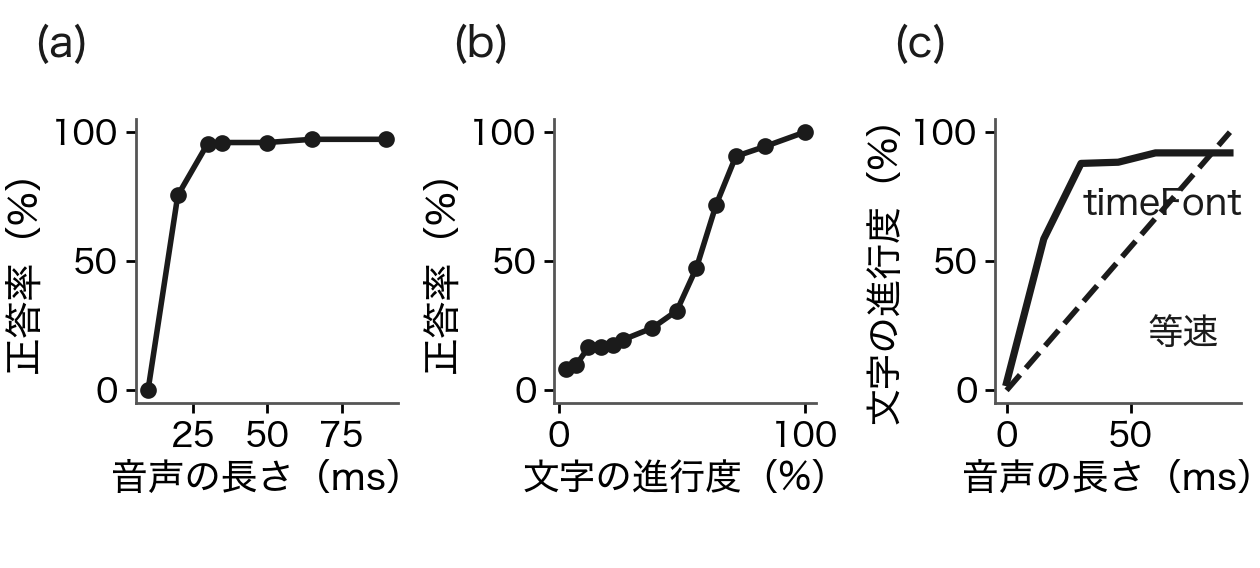
\includegraphics[width=\hsize]{fig/fig3_curves.png}
\end{center}
\caption{代表文字「あ」について，(a) 音声を時刻 $t$ で打ち切ったときの正答率，(b) 文字アニメーションを進行度 $s$ で打ち切ったときの正答率（ぼかし解除方式），(c) その 2 つから求めた進行度（実線）と，比較のための等速（破線）を示す．}
\label{fig:curves}
\end{figure}

\subsection{生成結果の確認}

8 文字 × 4 方式 × 7 打ち切り時点について，生成した進行度を視覚の対応曲線に代入し直したところ，目標との差は平均 2.1 パーセントポイントであった．ただし，生成と確認に同じ曲線を用いているため，これは式 (1) どおりに動作することの確認である．


\section{作成した timeFont の評価}

表示方式と対応づけの方法によって，生成された表示に対する主観的な評価がどのように変わるかを確かめる．4つの表示方式と4つの対応づけの方法を組み合わせた16条件を用意し，表示方式または対応づけの方法の一方だけが異なる組を一対比較した．ここでは，それぞれの動きの自然さと好ましさを評価した．対応づけの方法は，用いる量を正答率と情報量の 2 種類，合わせ方を全時点と中点のみの 2 種類とし，これらを組み合わせた 4 条件とした．ここでいう中点とは，その量が測定された最小値と最大値のちょうど中間の値に達する最初の時刻である．すなわち，各時点の正答率を一致させる正答率条件，各時点の情報量を一致させる情報量条件，正答率が中点に達する時刻のみを一致させてそのあとは等速で進める条件，および情報量が中点に達する時刻のみを一致させてそのあとは等速で進める条件である．ここでいう情報量は，回答の分布から求めた KL ダイバージェンスである．これは 2 つの離散分布の隔たりを測る指標である．回答した文字を R，提示した文字を c，提示水準を j として，c を j で提示したときの回答分布 P(R | c, j) が，同じ水準で全文字をまとめた回答分布 P(R | j) からどれだけ離れているかをビット単位で求めた．正答に至らない回答であっても，回答が特定の文字に偏っていればこの値は大きくなる．比較する条件の組は，表示方式と対応づけの方法のうち一方のみが異なる 48 種類に限り，両方が同時に異なる組合せは除外した．各実験協力者には，48 種類のうち連続する 24 種類を割り当て，参加者間で各組の提示回数がそろうようにした．

実験協力者は Yahoo! クラウドソーシングで募集した 112 名であり，111 名が全試行を完了した．対応データの測定に参加した実験協力者は，この評価には参加していない．各実験協力者は，対象とした 8 文字について 3 回ずつ，計 24 回の比較を行った．各比較では，「動きが自然なのはどちらか」および「より好ましいのはどちらか」の 2 問に対し，A と B のいずれかを選択して回答する．引き分けの選択肢は設けなかった \cite{perez}．各比較における左右の配置は，実験協力者と試行の通し番号にもとづいて入れ替えた．表示の大きさ，提示位置，および消去の方法は測定と同じとした．アニメーションの変化が終わった状態を 34 ms 提示したのち消去した．この 34 ms は，画面の更新が最も遅い 30 Hz の端末でも最後のコマが 1 回は表示されるように取った値で，対応データを測ったときと同じである．その後，2 秒の空白をはさんで繰り返した．音声は提示していない．評価項目および比較条件の種類ごとに，8 文字を統合した二項検定を行った．96 件の比較をすべて実施し，Holm 法で補正した．あわせて，16 条件について Thurstone Case V の尺度値を求めた \cite{perez}．これは，どちらが選ばれたかの回数から，16 条件を 1 本の目盛りの上に並べ直す方法である．

合計 2,675 件の一対比較試行を得た．96 件の比較のうち，有意差が見られたものは 16 件であり（いずれも $p < 0.05$），そのうち 15 件は対応づけの方法のみが異なる組であった．表示方式のみが異なる比較で有意差が見られたのは，残る 1 件だけであった．選択率の差が最も大きかったのは，部分表示方式において，中点を正答率と情報量のいずれで一致させるかのみが異なる比較であり，63 件中 59 件（94\%）で情報量にもとづく条件が選択され，有意差が見られた（$p < 0.05$）．この 2 条件の違いを図 4 に示す．部分表示方式の「あ」では，正答率にもとづく対応づけで進行度が 7\% までしか進まないのに対し，情報量にもとづく対応づけでは 75\% まで進む．尺度値でも，情報量にもとづく条件が上位に，正答率にもとづく条件が下位に並び，その両端はいずれも部分表示方式であった．なお，尺度の両端を占めた部分表示方式は，4.8 節で述べたとおり，同じ進行度でも提示時間が長いほど正答率が高くなる．本研究の測定は，どの進行度も同じ速さで見せて行った．生成した表示では進む速さが時間によって変わるため，部分表示方式では，狙った正答率からのずれが他の方式より大きいと考えられる．文字の進む速さが変わっても使える対応データを作ることは今後の課題である．

提示時間は試行ごとに割り当てており，各実験協力者は両方の提示時間を経験している．ただし割り当ては通し番号にもとづく規則で決めており，無作為化していない．また，この結果は，他の 3 方式について提示時間の影響がないことを示すものではない．この結果から，部分表示方式の生成には 300 ms 条件のみを用いた．


\begin{figure}[tb]
\begin{center}
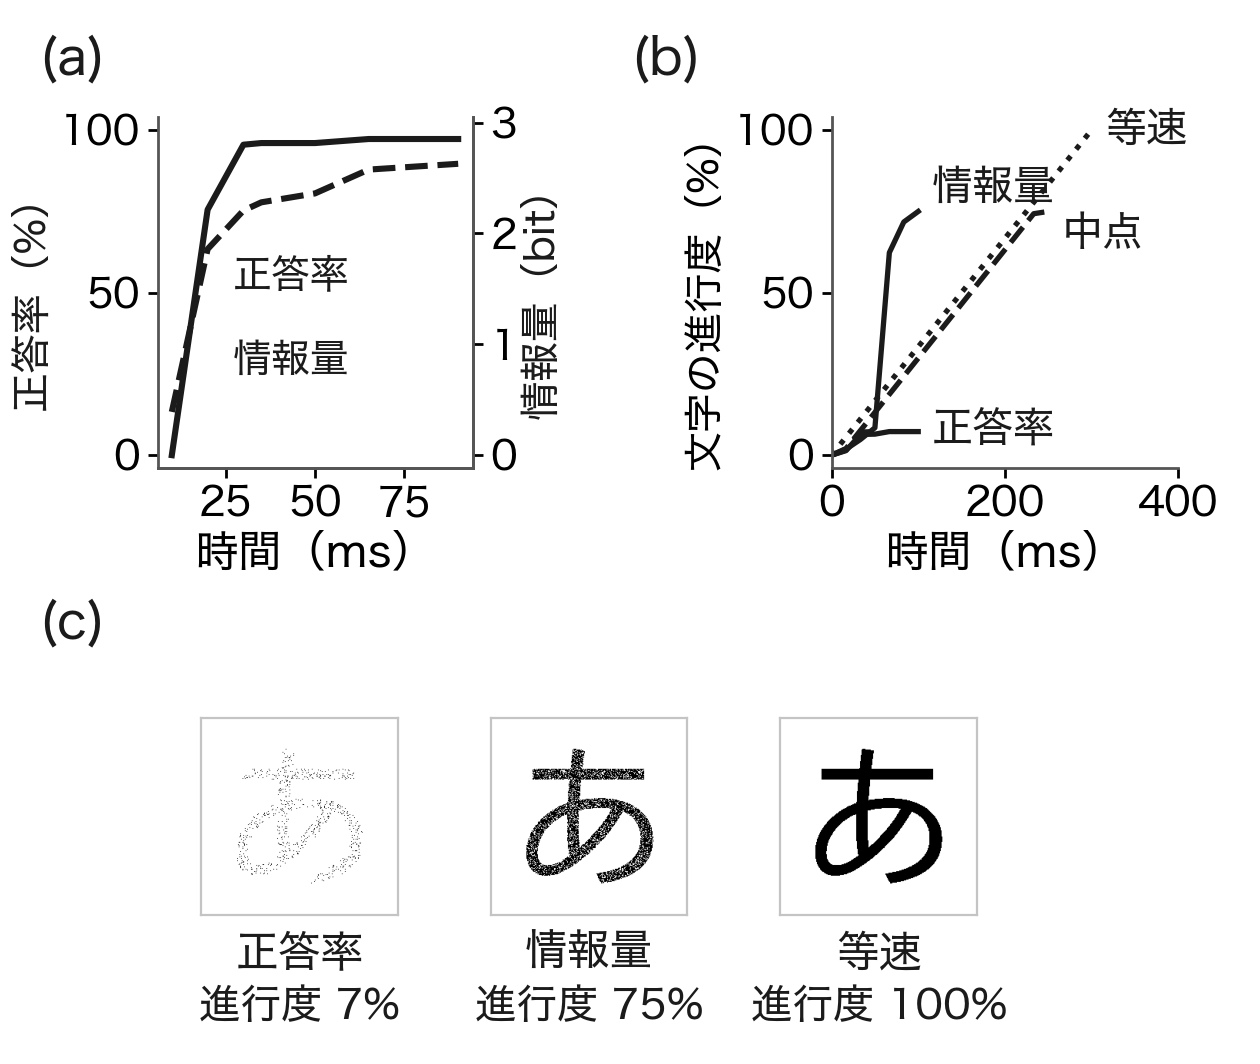
\includegraphics[width=\hsize]{fig/fig4_measures.png}
\end{center}
\caption{対応づけに用いる量による違い．部分表示方式の「あ」について，(a) 音声で測った正答率と情報量，(b) それを文字側に写した進行度，(c) 終わった時点の見え方を示す．}
\label{fig:measures}
\end{figure}

\section{timeFont を使うためのツールと実装例}


\subsection{アプリケーションと生成器}

生成システムは，入力を受け取る部分，正答率と進行度の対応データ，および生成器の 3 つからなる．対応データは，文字と表示方式の組ごとに，どの進行度でどれだけ当てられるかを持つ．生成器は，入力から得た時刻ごとの目標をこの対応データに照らし，その正答率になる進行度を求め，文字アニメーションを描いて音声と合成し，動画を出力する．

生成システムは，ブラウザ上で操作する画面をもつアプリケーションとして実装した（図 5）．入力方法，表示方式，対象とする文字，および 1 文字の長さを選んで生成すると，その場で動画を再生できる．生成処理の本体は Python で実装したエンコーダであり，音声トラックと文字アニメーションを合成した MP4 形式の動画を 60 fps で出力する．漢字とカタカナはひらがなに変換する．1 文字の長さは指定できるが，音声クリップ自体は伸縮せず，文字と文字の間隔が変わる．描画の条件は測定時と生成時でそろえた．同じ生成機能はコマンドラインからも呼び出せる．MCP サーバも用意しており，対話型 AI から文字列を渡して動画を得ることもできる．


\begin{figure}[tb]
\begin{center}
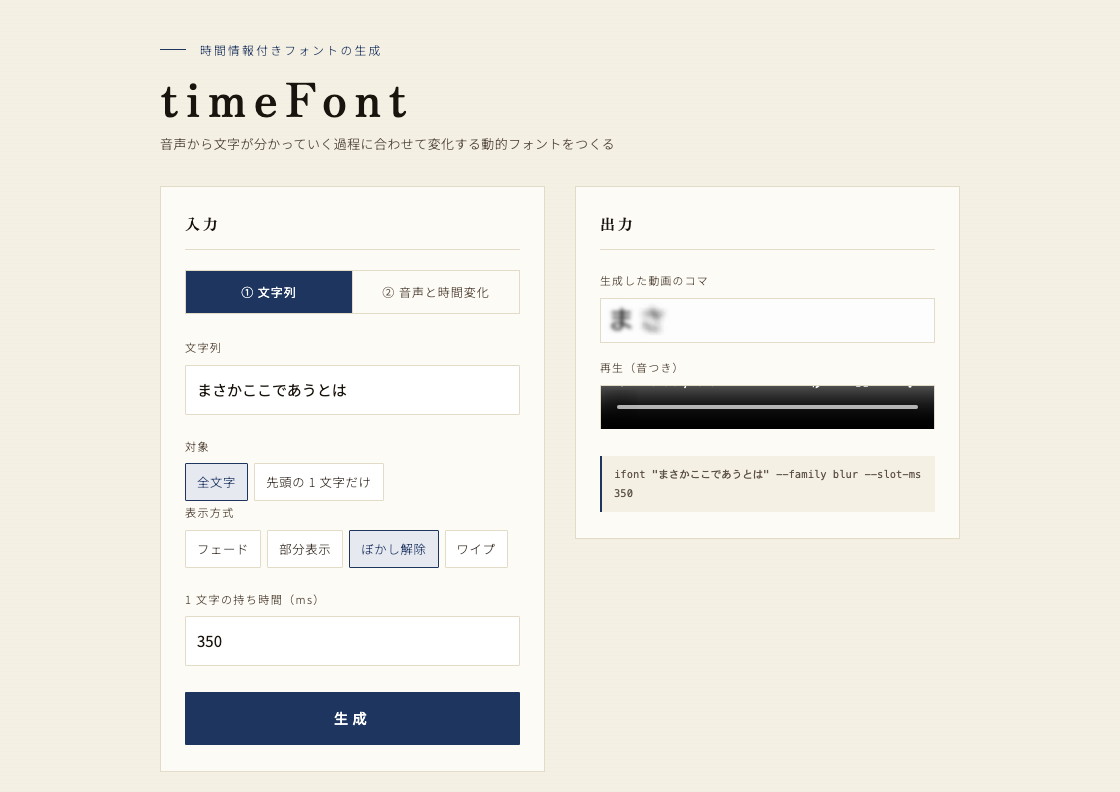
\includegraphics[width=0.72\hsize]{fig/fig5_app.png}
\end{center}
\caption{生成システムのアプリ画面．文字列を入力して生成した直後の状態である．}
\label{fig:app}
\end{figure}

\subsection{入力方法と動作例}

生成システムには 2 通りの入力方法がある．1 つは，かなの文字列を入力する方法である．この場合，測定に用いた音声クリップと対応データから音声と timeFont を生成する．台詞の字幕のように全文字の識別が問題となる場合は全文字を対象とする．例として「まさかここであうとは」の 10 文字すべてを，ぼかし解除方式で生成した動画を作成した．一部の文字だけを対象にすることもできる．いろはかるたでは第 1 音によって札が一意に定まるため，第 1 音のみを対象とし，残りの文字は読み上げられた時刻に表示する．

もう 1 つは，音声，各文字の開始時刻，および識別の時間変化を外部から入力する方法である．この場合は，与えられた時間変化に合わせて timeFont を生成する．例として，競技かるたで実測した決まり字の識別時刻 \cite{maruyama} から，各時刻までに札を識別した選手の割合を求め，字幕を生成した．この値は本研究で測定した正答率とは異なるため，外部から与える目標の時間変化として用いた．読み上げ音声には，その測定で用いた音声をそのまま入力した．


\section{今後の展望}


本研究で十分な試行数で対応データを測定したのは 8 文字である．今後は，対応データを全かなに広げるとともに，音声の速度を変えた場合にも，その速度に合わせて timeFont を生成できるようにしたい．


